\label{chap:intro}
\section{Background and Motivation}
The proliferation of Large Language Models (LLMs) has fundamentally transformed enterprise automation, progressing from static conversational agents to autonomous, tool-executing systems operating in Retrieval-Augmented Generation (RAG) paradigms \cite{lewis2020retrieval}. Under enterprise RAG architectures, generative models do not rely exclusively on internal pre-trained parametric memory. Instead, external vector databases (such as ChromaDB, Pinecone, or FAISS) dynamically store high-dimensional embeddings of internal proprietary documents, compliance guides, customer records, and operational manuals. When a user submits an instruction, semantic retrieval algorithms execute nearest-neighbor queries across the vector store to extract relevant context chunks, synthesizing an augmented prompt for the downstream LLM.

Despite these efficiency gains, vector-augmented agentic architectures possess a critical, systemic architectural flaw: \textbf{vector retrieval is purely syntactic and proximity-based}. High-dimensional distance calculations (such as cosine similarity or inner product) evaluate mathematical vector alignment without evaluating semantic intent, data provenance, or safety constraints. Consequently, adversaries can exploit this blind spot through \textit{Indirect Prompt Injection} (IPI) and vector store poisoning attacks \cite{zou2025poisonedrag, greshake2023not}.

\section{Problem Statement}
In an Indirect Prompt Injection threat vector, an adversary does not attack the conversational chat box directly. Rather, they deposit malicious, command-hijacking instructions within third-party files—such as PDF resumes, vendor invoices, or public forum posts—that are ingested by automated document processing pipelines. When an authorized enterprise employee queries the assistant, the retrieval engine innocently pulls the adversary's poisoned chunk based on topical overlap. 

Once loaded into the active LLM context window, the hidden command sequence executes with the assistant's elevated enterprise permissions. Documented exploits include unauthorized financial wire transfers, database connection string exfiltration, administrative credential theft, and API token hijacking.

Current commercial industry defenses depend on \textit{Generative Guardrail LLMs} (such as Meta Llama Guard \cite{inan2023llama} or NVIDIA NeMo Guardrails). While semantically expressive, these models create severe bottlenecks for production adoption:
\begin{enumerate}
    \item \textbf{Prohibitive Latency Penalty:} Calling a secondary 7B--13B parameter LLM for every retrieved document chunk introduces $800$\,ms to $2500$\,ms of latency, severely degrading user experience and conversational responsiveness.
    \item \textbf{Token Consumption Costs:} Processing thousands of candidate enterprise chunks through generative guardrails inflates cloud API token expenditure exponentially.
    \item \textbf{Catastrophic Hard Refusal:} When conventional guardrails flag an injection, they typically terminate the entire agent pipeline with a rigid exception (\enquote{I cannot answer this request}), completely halting valid user workflows.
\end{enumerate}

\section{Research Objectives}
To resolve these foundational vulnerabilities, this thesis introduces \textbf{Vector-Shield}: a dual-stage, hybrid Neuro-Symbolic middleware architecture engineered to operate directly on multi-dimensional embedding vectors before context reaches the LLM. The core research objectives comprise:
\begin{enumerate}
    \item \textbf{Sub-2ms Deterministic Outlier Interception:} Develop an angularly calibrated Local Outlier Factor (LOF) formulation coupled with dimensionality reduction to intercept obvious and catastrophic vector anomalies in less than $2.0$\,ms.
    \item \textbf{Deep Borderline Sequence Classification:} Train and integrate a high-capacity ModernBERT transformer encoder (149M parameters) fine-tuned on an NVIDIA A100 GPU cluster to classify stealthy and obfuscated borderline payloads ($1.30 < \text{LOF} < 2.50$) with $100\%$ precision.
    \item \textbf{Stateful Cyclic Self-Healing Recovery:} Implement a compiled LangGraph workflow that automatically purges poisoned vectors, rewinds agent state, and queries alternative authenticated chunks without human intervention or conversational failure.
    \item \textbf{Production Enterprise Tooling:} Construct a full-featured Streamlit Security Cockpit incorporating 3D PCA vector space projections, live attack simulation, dynamic document ingestion validation, and SIEM incident alerting.
\end{enumerate}

\begin{figure}[h]
\centering
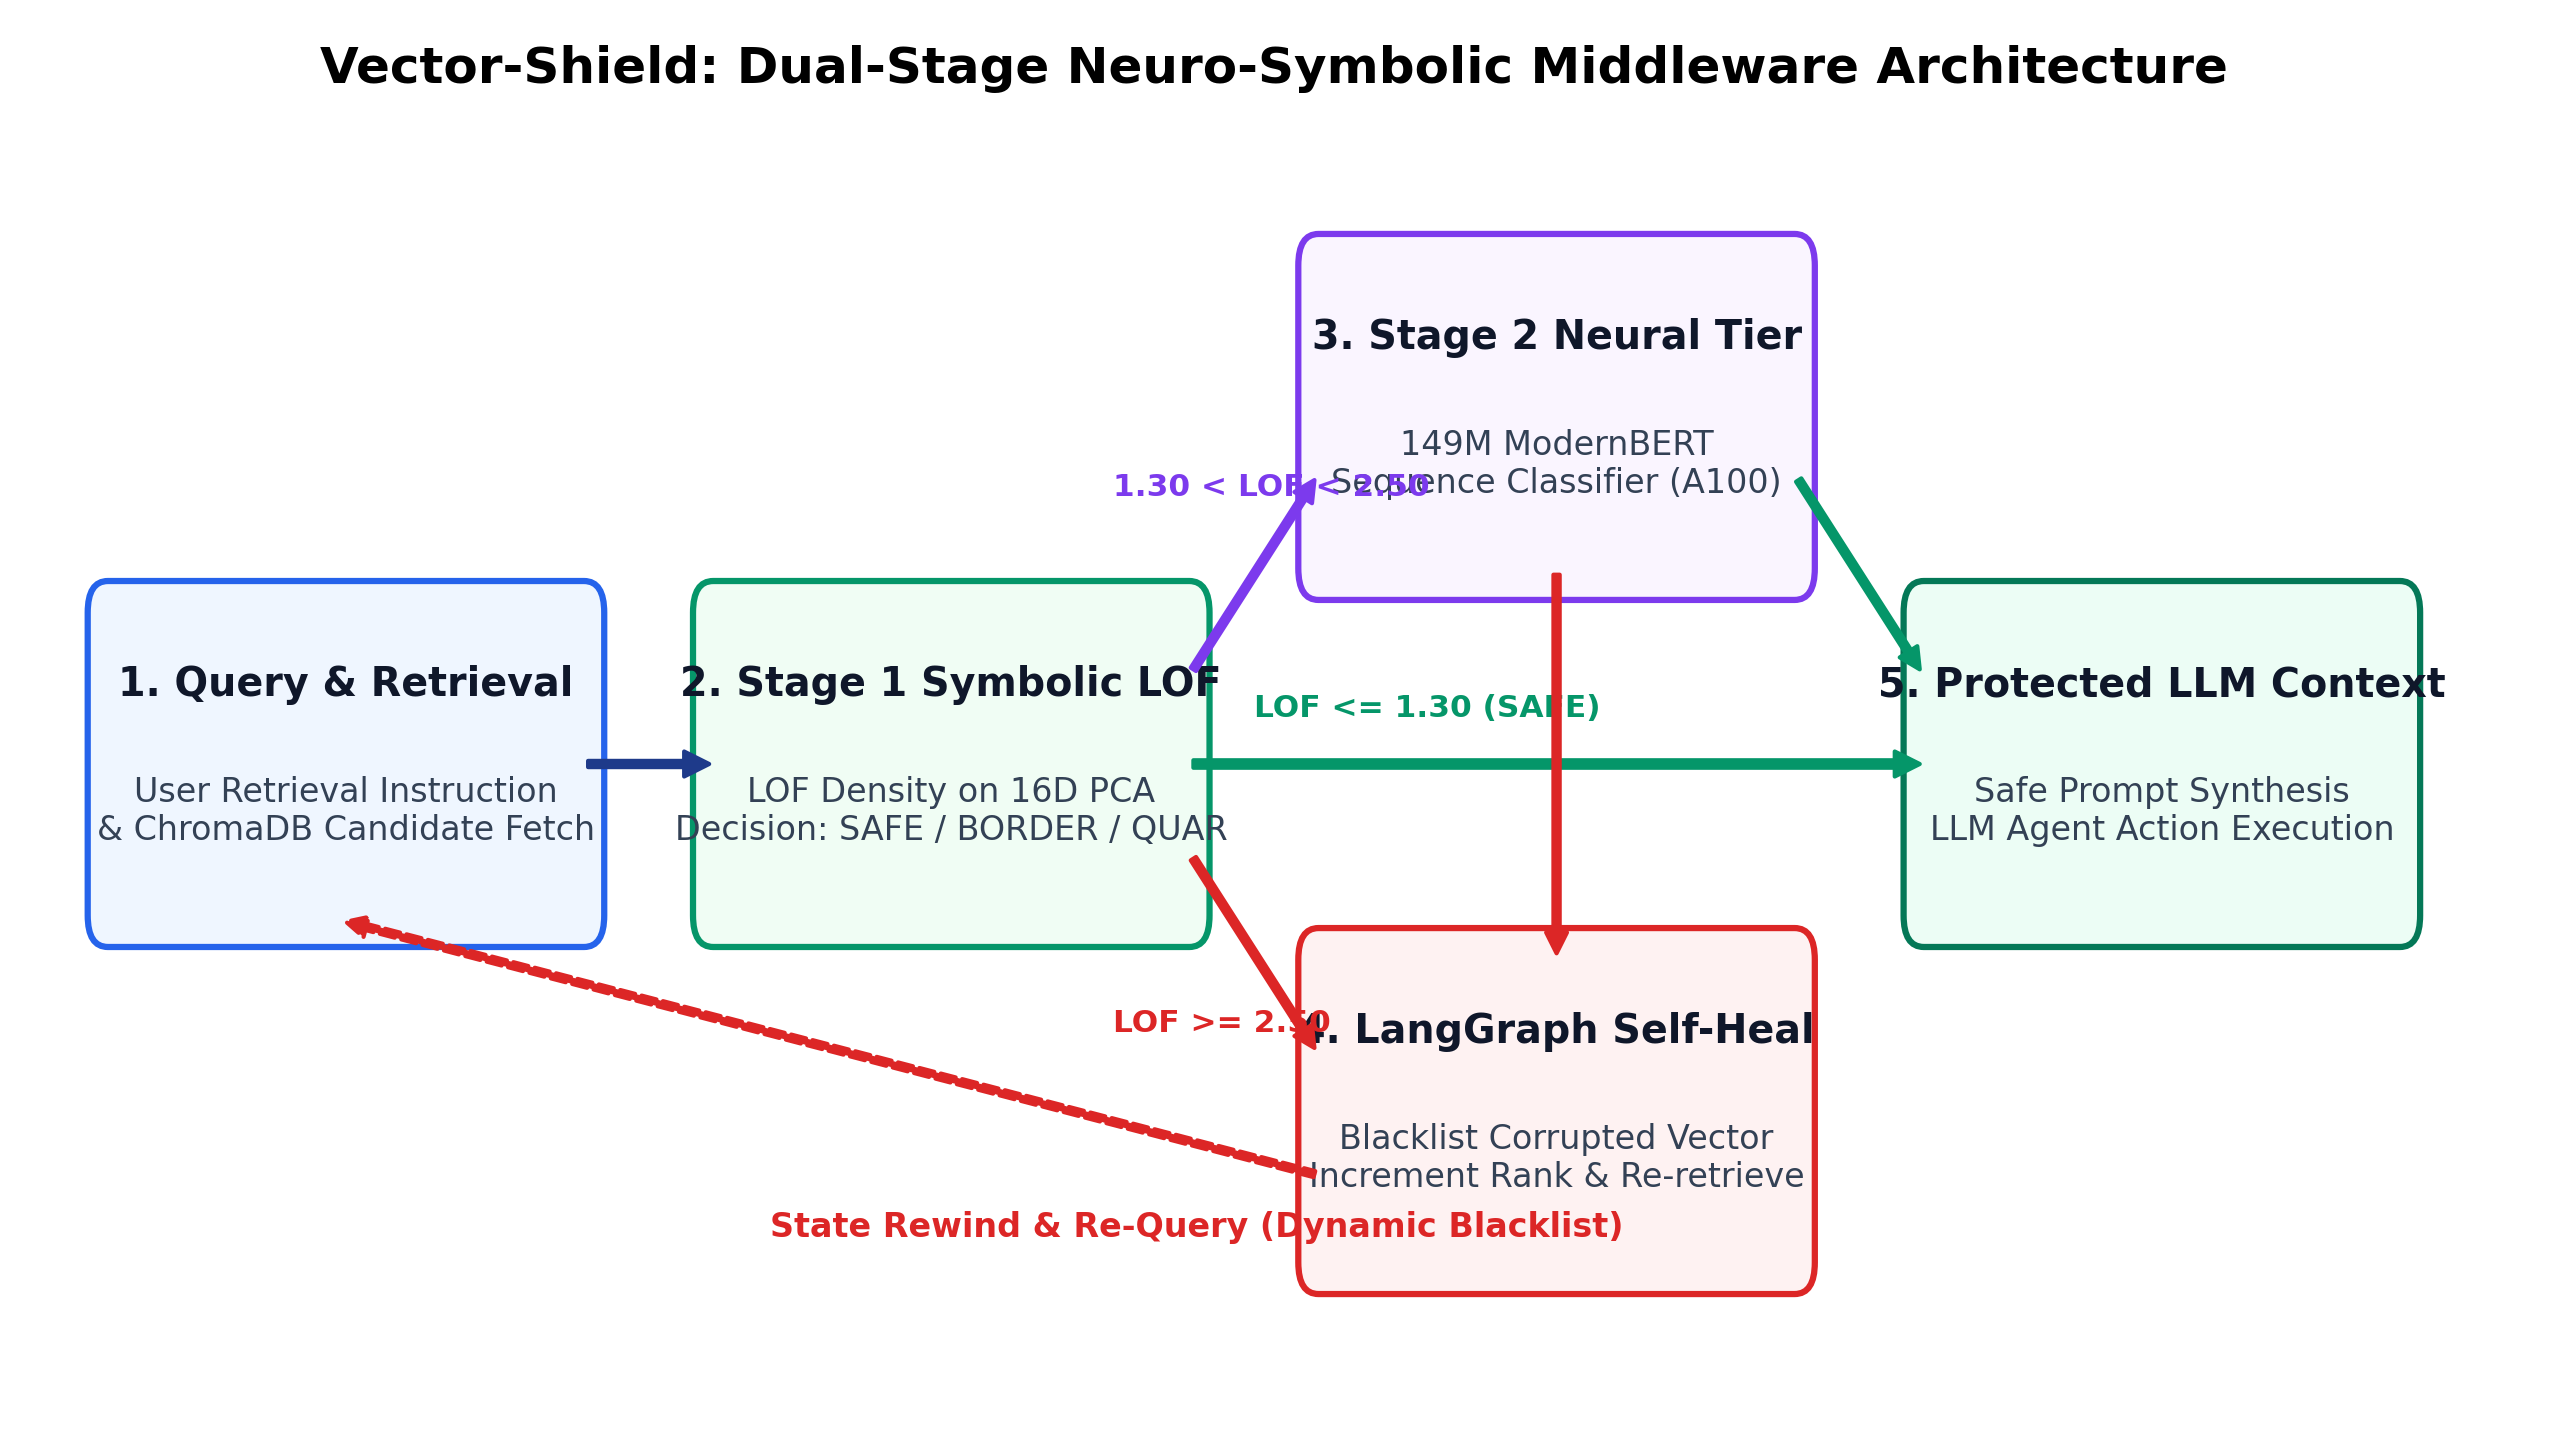
\includegraphics[width=0.92\textwidth]{architecture_diagram.png}
\caption{Dual-Stage Neuro-Symbolic Middleware Architecture of Vector-Shield}
\label{fig:architecture_diagram}
\end{figure}

\section{Thesis Organization}
The remainder of this thesis is structured as follows:
\begin{itemize}
    \item \textbf{Chapter 2 (Literature Review)} surveys existing literature on RAG architectures, indirect prompt injection vectors, spatial anomaly detection, and transformer guardrails.
    \item \textbf{Chapter 3 (Threat Modeling \& Problem Formulation)} formalizes the mathematical threat surface, attack taxonomy, and geometric intuition behind vector space manipulation.
    \item \textbf{Chapter 4 (Stage 1: Symbolic Geometric Interceptor)} presents the mathematical derivation of our angularly scaled LOF interceptor and adaptive PCA projection.
    \item \textbf{Chapter 5 (Stage 2: ModernBERT Neural Sequence Classifier)} details the fine-tuning methodology, FP16 training optimization on NVIDIA A100 GPUs, and inference latency benchmarks.
    \item \textbf{Chapter 6 (Stateful Self-Healing Orchestration with LangGraph)} explores the state machine architecture, graph node definitions, and self-recovery logic.
    \item \textbf{Chapter 7 (Empirical Results, Evaluation \& Security Cockpit)} provides empirical evaluation across real-world datasets (NVIDIA Garak, HuggingFace) and demonstrates the interactive security cockpit.
    \item \textbf{Chapter 8 (Conclusion and Scope for Further Research)} synthesizes our findings and delineates future research vectors toward enterprise zero-trust AI architectures.
\end{itemize}
